\documentclass[11pt,letterpaper]{article}
\usepackage[T1]{fontenc}
\usepackage{lmodern}
\usepackage[margin=1in]{geometry}
\usepackage{microtype}
\usepackage{amsmath,amssymb,amsthm,mathtools}
\usepackage{booktabs,longtable,array,enumitem}
\usepackage{xcolor}
\usepackage{tikz}
\usetikzlibrary{arrows.meta,angles,quotes}
\usepackage{listings}
\usepackage{fancyhdr}
\usepackage[colorlinks=true,linkcolor=blue!45!black,citecolor=blue!45!black,urlcolor=blue!45!black,breaklinks=true]{hyperref}
\usepackage[nameinlink,noabbrev]{cleveref}
\setlength{\headheight}{14pt}
\pagestyle{fancy}
\fancyhf{}
\lhead{Constructive Gauss--Bonnet in iPRA}
\rhead{\thepage}
\renewcommand{\headrulewidth}{0.3pt}
\setlength{\parskip}{0.35em}
\setlength{\parindent}{1.3em}
\setlist{itemsep=0.25em,topsep=0.35em}
\newtheorem{theorem}{Theorem}[section]
\newtheorem{lemma}[theorem]{Lemma}
\newtheorem{proposition}[theorem]{Proposition}
\newtheorem{corollary}[theorem]{Corollary}
\theoremstyle{definition}
\newtheorem{definition}[theorem]{Definition}
\newtheorem{remark}[theorem]{Remark}
\newcommand{\ipra}{\ensuremath{\mathrm{iPRA}}}
\newcommand{\PR}{\ensuremath{\mathrm{PR}}}
\newcommand{\Q}{\mathbb Q}
\newcommand{\N}{\mathbb N}
\newcommand{\Z}{\mathbb Z}
\newcommand{\R}{\mathbb R}
\newcommand{\dd}{\,\mathrm d}
\newcommand{\eps}{\varepsilon}
\newcommand{\Del}{\Delta}
\newcommand{\abs}[1]{\left|#1\right|}
\newcommand{\norm}[1]{\left\|#1\right\|}
\newcommand{\At}{\operatorname{At}}
\newcommand{\ceilLog}{\operatorname{clog}_2}
\newcommand{\Eval}{\operatorname{Eval}}
\newcommand{\code}[1]{\texttt{\detokenize{#1}}}
\newcommand{\repo}{\texttt{ProveIt}}
\newcommand{\status}[1]{\par\noindent\fcolorbox{blue!30!black}{blue!3}{\parbox{0.94\linewidth}{#1}}\par}
\lstset{basicstyle=\ttfamily\small,breaklines=true,columns=fullflexible,frame=single,rulecolor=\color{black!20}}
\hypersetup{pdftitle={Constructive Gauss--Bonnet in intuitionistic primitive recursive arithmetic},pdfauthor={Research report prepared for Vladimir Reshetnikov}}
\begin{document}
\hypersetup{pageanchor=false}
\begin{titlepage}
\vspace*{0.65in}
{\Large\color{blue!45!black} Constructive geometry and weak arithmetic\par}
\vspace{0.5in}
{\huge\bfseries Constructive Gauss--Bonnet\par}
\vspace{0.14in}
{\LARGE in intuitionistic primitive recursive arithmetic\par}
\vspace{0.45in}
{\large A quantitative proof for explicitly presented compact surfaces,\par
including boundary, corners, and nonorientable surfaces\par}
\vspace{0.55in}
{\large Prepared for Vladimir Reshetnikov\par}
{\large November 21, 2026\par}
\vfill
\status{\textbf{Verification status.} This report gives a human-readable proof of a fixed-program \ipra\ theorem schema, together with exact finite arithmetic certificates, executable examples, and a Lean formalization plan. The new Lean files are \emph{uncompiled candidates}; a complete kernel-checked Gauss--Bonnet derivation is not claimed. Existing \repo\ source is inspected at commit \texttt{d36b35eed5bd01af4ade66bf539622495813ccc8}.}
\vspace{0.2in}
\end{titlepage}
\hypersetup{pageanchor=true}
\begin{abstract}
We prove Gauss--Bonnet for a finite triangulated surface whose metric and local compatibility data are supplied by primitive recursive rational names, quantitative $C^2$ jets, and explicit nondegeneracy margins. The conclusion is a family of rational error inequalities provable using intuitionistic logic and quantifier-free induction. Its usual mathematical interpretation is
\[
\int_M K\dd A+\int_{\partial M}k_g\dd s+
\sum_{v\in\partial M}(\pi-\alpha_v)=2\pi\chi(M).
\]
The boundary convention uses the inward conormal and therefore does not require global orientability. A more general identity includes seam curvature and cone defects for independently specified triangle metrics.

The local proof uses an upper triangular orthonormal coframe. On the three fixed sides of the reference triangle, three explicit arctangent branches make the total turning identity telescope. A finite rectangular grid proves the required Green identity with an explicit error bound. Thus no general turning theorem, geodesic triangulation construction, unbounded search, choice principle, or abstract compactness argument is needed. We explain exactly which data replace those existence arguments, how every loop uses a quantifier-free invariant, and which additional Lean modules would complete an object-level derivation in \repo's calculus.
\end{abstract}
\tableofcontents
\newpage
\section{The result and its scope}\label{sec:result}

The constructive difficulty is not the final Euler-characteristic calculation. It is justifying the local curvature formula, the integration rules, and the finite geometric presentation within a theory whose induction is restricted to quantifier-free formulas. We address these separately, then combine their quantitative statements.

\begin{theorem}[Constructive smooth Gauss--Bonnet]\label{thm:main}
Fix primitive recursive programs for the data described in \cref{sec:data}. Let $d$ be numerical parameters supplying:
\begin{enumerate}
\item a finite triangulated compact two-dimensional manifold, possibly disconnected, with boundary allowed;
\item on each reference triangle, a positive definite $C^2$ metric given by regular rational names for an upper triangular coframe and its jets through order two;
\item primitive recursive moduli of continuity and differentiability, and rational lower bounds for every denominator used;
\item compatible metric charts across interior edges and at vertices, including finite certificates that the vertex sectors occur once in the correct circular or interval order.
\end{enumerate}
Then there are explicitly described primitive recursive rational quadrature programs for curvature, boundary geodesic curvature, and corner turns. For every precision $n$ they satisfy the rational Gauss--Bonnet error bound in \cref{thm:arith}. The corresponding equality of regular names is
\begin{equation}\label{eq:main}
\boxed{\quad
\sum_T\int_T K\dd A+
\sum_{e\subset\partial M}\int_e k_g\dd s+
\sum_{v\subset\partial M}\tau_v
=2\pi\bigl(V-E+F\bigr).\quad}
\end{equation}
Here $\tau_v=\pi-\alpha_v$, where $\alpha_v\in(0,2\pi)$ is the total interior boundary angle, and $k_g=g(\nabla_TT,n_{\mathrm{in}})$ uses the inward unit conormal. At a smooth boundary vertex $\tau_v=0$. Global orientability is unnecessary.

For each fixed suite of the primitive recursive programs, the numerical assertion is a theorem schema of \ipra\ from the stated presentation hypotheses. The algorithm is uniform in numerical parameters, the number of triangles, and precision.
\end{theorem}

The schema qualification is essential. First-order arithmetic does not quantify over an arbitrary real manifold or an arbitrary function $\N\to\Q$. It quantifies over natural-number parameters of fixed programs, or over finite certificates. Nor is there a single primitive recursive evaluator for every primitive recursive program. An optional alternative is a coded evaluator with an explicitly supplied primitive recursive time bound; the bound then belongs to the input contract.

\begin{theorem}[Piecewise smooth form]\label{thm:piecewise_intro}
For a finite triangulated surface with independently presented positive $C^2$ triangle metrics, write
\[
C_T=\int_TK\dd A,\qquad
G_{T,e}=\int_e k_{g,T}\dd s,\qquad
\alpha_{T,v}=\text{the interior angle of triangle $T$ at $v$}.
\]
For an interior edge $e=T\cap T'$, set $J_e=G_{T,e}+G_{T',e}$. For an interior vertex set $D_v=2\pi-\sum_{T\ni v}\alpha_{T,v}$; for a boundary vertex set $\tau_v=\pi-\sum_{T\ni v}\alpha_{T,v}$. Then
\begin{equation}\label{eq:piecewise}
\sum_T C_T+\sum_{e\text{ interior}}J_e+
\sum_{e\text{ boundary}}G_e+
\sum_{v\text{ interior}}D_v+
\sum_{v\text{ boundary}}\tau_v=2\pi\chi.
\end{equation}
This is an equality of effective names, with a finite rational error version. If edge metrics agree on their tangential restrictions, it describes the corresponding glued piecewise Riemannian metric. The algebraic identity itself only needs the individual triangle metrics and the finite incidence data.
\end{theorem}

The smooth theorem follows because a common smooth metric makes $J_e=0$, and a one-turn tangent fan makes $D_v=0$. These facts are proved from local compatibility data in \cref{sec:gluing}; neither Gauss--Bonnet nor the desired angle-sum identities are assumed as metric hypotheses.

For closed smooth surfaces, \eqref{eq:main} reduces to $\int_MK\dd A=2\pi\chi$. For Euclidean triangle metrics, \eqref{eq:piecewise} reduces to the angle-defect theorem. For a supplied geodesic triangle, the local theorem gives angle excess. Thus the smooth result contains genuine differential geometry; it is not merely a renaming of the polyhedral identity.

\subsection{What has changed from a classical statement}

Classical accounts begin with a compact Riemannian surface and obtain triangulations, chart refinements, and bounds by existence arguments; see, for example, the local and global treatments in \cite{new,shifrin}. Here these finite presentations and bounds are supplied. We do not claim that \ipra\ constructs an effective triangulation of every abstract compact surface, extracts moduli from qualitative $C^2$ continuity, or turns every externally computable metric into a primitive recursive one.

This is a substantive constructive theorem for a broad explicitly represented class. In particular, a finite smooth triangulation with rational/algebraic/elementary chart formulas and certified margins supplies the required kind of input whenever those formulas have the stated effective bounds. The sphere-octant example in \cref{sec:examples} exhibits nonzero curvature and verifies the local identity independently by elementary integration.

\subsection{The logical endpoint}

We use \ipra\ with natural numbers, a symbol and defining equations for every primitive recursive function, intuitionistic first-order logic with equality, the successor axioms, and quantifier-free induction. Integers, rationals, lists, and finite matrices are numerical codes. The assertion ``this proof lies in \ipra'' means that the finite numerical lemmas have derivations using only those rules; it does not mean that a Lean theorem about Mathlib's real numbers has that strength.

The report supplies a human proof and a concrete construction of the relevant primitive recursive bounds. The new Lean material separates an ambient rational algebra layer, a small proposed object-calculus bridge, and the still-to-be-implemented analytic derivations. The exact scope of each is recorded in \cref{sec:lean} and in the archive's verification notes.

\section{Numerical and geometric presentation data}\label{sec:data}

\subsection{Codes, regular names, and the meaning of an inequality}

Encode an integer by a sign and a natural magnitude, and a rational by an integer numerator and a positive natural denominator. Normalization by a greatest common divisor is optional. Addition, multiplication, sign comparison, bounded list access, and denominator clearing are primitive recursive. Every rational inequality used below is a decidable relation on such codes, hence has a primitive recursive Boolean characteristic function.

A \emph{regular rational name} is a fixed primitive recursive rational-valued function $r(d,k)$, with a proof or hypothesis of
\begin{equation}\label{eq:regular}
\abs{r(d,k)-r(d,l)}\le 2^{-k}+2^{-l}\qquad(k,l\in\N).
\end{equation}
We write its interpreted value as $r(d)$. This notation is eliminable: in the usual completion it is approximated by $r(d,k)$ within $2^{-k}$. Conversely, a quadrature algorithm whose outputs approximate a fixed integral with that bound gives such a name, by comparison through finite common refinements; an independently constructed completion is not required inside arithmetic.

For example, $\abs{x-y}\le b$, with rational $b\ge0$, can be read arithmetically as
\[
\forall k\quad\abs{x(k)-y(k)}\le b+2^{1-k}.
\]
When a polynomial or quotient expression is involved, its input errors are first propagated by the explicit bounds below. We do not compare unknown real values for equality to decide a branch. Branches used by programs compare rational approximations with a supplied nonzero margin, or compare natural numbers. All claims about real names in this report are abbreviations for this type of first-order numerical assertion.

\subsection{Effective jets}

Let $U$ be a fixed rational polygonal domain, such as a triangle with a small rational collar. A quantitative $C^r$ name for $f$ consists of rational evaluators
\[
f_\nu(z,k)\quad (z\in U\cap\Q^2,\ |\nu|\le r),
\]
where $\nu=(\nu_1,\nu_2)$ is a multi-index, together with:
\begin{enumerate}
\item regular-name contracts for every jet value, uniformly in $z$;
\item a rational bound $H\ge1$ for the absolute values of the jets;
\item a common modulus $\mu$ such that
\begin{equation}\label{eq:continuitycontract}
\norm{z-w}_1\le2^{-\mu(q)}
\quad\Longrightarrow\quad
\abs{f_\nu(z)-f_\nu(w)}\le2^{-q};
\end{equation}
\item a common differentiability modulus $\lambda$ such that, for $|\nu|<r$ and a segment contained in $U$,
\begin{equation}\label{eq:jetcontract}
\begin{split}
\norm{h}_1\le2^{-\lambda(q)}\quad\Longrightarrow\quad
\abs{f_\nu(z+h)-f_\nu(z)
-\sum_{j=1}^2f_{\nu+e_j}(z)h_j}
\le2^{-q}\norm{h}_1.
\end{split}
\end{equation}
\end{enumerate}
The programs for $\mu$ and $\lambda$ are fixed PR programs, possibly depending on numerical parameters $d$. We replace them by their bounded running maxima when monotonicity is useful. Mixed derivatives use one shared multi-index entry, so the second-order data include the required equality of mixed partials.

The finite-precision translation of \eqref{eq:jetcontract}, using all input values at precision $k$, adds at most $(2+\norm{h}_1)2^{-k}$ to its right-hand side. The translation of \eqref{eq:continuitycontract} adds $2^{1-k}$. These are explicit arithmetic formulas. They are hypotheses about the input functions; a finite mesh checker cannot decide their truth at every precision. An application can either work under them or supply separate \ipra\ derivations for its concrete formulas.

The derivative contract is quantitative differentiability, not a disguised integration theorem. Products and reciprocals preserve it by finite algebra; a detailed operation rule is given in \cref{sec:bounds}. Thus one may present the initial coframe by elementary formulas and derive the contracts instead of listing unrelated functions and assuming their calculus. A composition evaluated at a named point is computed by first taking a rational approximation to that point at the outer function's supplied modulus. The rational collar and overlap margins ensure that the approximation remains in the evaluation domain; they are part of the chart data.

\subsection{Finite surfaces}

\begin{definition}[Certified triangulated surface]\label{def:mesh}
A surface mesh is a finite abstract simplicial complex with explicitly enumerated vertices, edges and triangular faces, satisfying the following decidable conditions.
\begin{enumerate}
\item Every face has three distinct vertices, every listed edge or vertex belongs to a face, and no face is duplicated.
\item Each edge belongs to one or two faces. An edge of degree one is a boundary edge.
\item The link of each vertex is a connected finite cycle or a connected finite path. Cycle links define interior vertices; path links define boundary vertices.
\end{enumerate}
Link cycles and paths can be supplied as lists of their vertices and edges, with a finite permutation certificate matching the incidence lists. Equivalently, a bounded traversal verifies them. No orientability certificate is required.
\end{definition}

These hypotheses exclude a singular vertex with a disconnected link, even if every edge has degree one or two. They describe the precise finite topological information used. Let $V_i,V_b,E_i,E_b,F$ be the numbers of interior vertices, boundary vertices, interior edges, boundary edges, and faces. Define
\[
V=V_i+V_b,\qquad E=E_i+E_b,\qquad\chi=V-E+F\in\Z.
\]
Connectedness and the classification of surfaces are not needed. In particular, we never replace $\chi$ by $2-2g$ using an unproved classification theorem.

\begin{lemma}[Incidence identities]\label{lem:incidence}
Every certified surface mesh satisfies
\begin{equation}\label{eq:incidence}
3F=2E_i+E_b,\qquad E_b=V_b,
\qquad 2\chi=2V_i+V_b-F.
\end{equation}
\end{lemma}
\begin{proof}
Enumerate the $3F$ face-side occurrences. Each interior edge accounts for two and each boundary edge for one, giving the first identity. A path link has exactly two endpoints, corresponding to the two boundary edges at its vertex. A cycle link has none. Counting boundary edge endpoints gives $2E_b=2V_b$, whence the second identity by cancellation in natural arithmetic. Substitution into $2(V_i+V_b-E_i-E_b+F)$ gives the third identity.

Each count is a finite sum. To justify it in \ipra, traverse the occurrence list while keeping the running number of incidences as a PR fold; induction on the processed length uses only an equality of natural-number expressions. The path/cycle certificates supply the local degree equations. Thus the proof uses quantifier-free induction even when the size of the mesh is variable.
\end{proof}

\subsection{The basic metric input}

Use the reference triangle
\[
\Del=\{(x,y)\in\R^2:x\ge0,\ y\ge0,\ x+y\le1\},
\quad A=(0,0),\ B=(1,0),\ C=(0,1).
\]
For each face supply $C^2$ names for $a,b,c$ on a rational collar of $\Del$, with
\begin{equation}\label{eq:Hbounds}
H^{-1}\le a,c\le H,\qquad
\abs{\partial^\nu a},\abs{\partial^\nu b},\abs{\partial^\nu c}\le H
\quad(|\nu|\le2).
\end{equation}
A finite maximum permits one common integer $H\ge1$ and common moduli for all faces. Set
\begin{equation}\label{eq:coframe}
\vartheta^1=a\dd x+b\dd y,
\qquad \vartheta^2=c\dd y,
\qquad g=(\vartheta^1)^2+(\vartheta^2)^2.
\end{equation}
In coordinates,
\[
g=\begin{pmatrix}a^2&ab\\ab&b^2+c^2\end{pmatrix},
\qquad \sqrt{\det g}=ac>0.
\]
The matrix $B_g=\left(\begin{smallmatrix}a&b\\0&c\end{smallmatrix}\right)$ converts a coordinate tangent vector to its orthonormal components.

This presentation loses no positive definite $C^2$ metric for which the requisite effective bounds are supplied. For
$g=\left(\begin{smallmatrix}E&F_0\\F_0&G\end{smallmatrix}\right)$, take
\[
a=\sqrt E,\qquad b=F_0/\sqrt E,\qquad
c=\sqrt{(EG-F_0^2)/E}.
\]
Rational positive lower bounds for $E$ and $EG-F_0^2$, upper bounds for the jets, and their PR moduli yield coframe bounds by the elementary operations in \cref{sec:bounds}. The symbol $F_0$ here is a metric coefficient and is unrelated to the number $F$ of faces.

\subsection{Smooth compatibility, including the vertex fan}\label{sec:compatibilitydata}

For the general piecewise formula no smooth compatibility is needed. For the smooth theorem we require an effective triangulated atlas, or the following local data it supplies.

\paragraph{Edge data.}
The two incident triangle collars are mapped into one common coordinate patch with a positive $C^2$ metric $h$. A full atlas may be taken quantitatively $C^3$, with supplied inverse charts and rational overlap margins; only its two-jet is used in the seam proof. The maps have nonsingular Jacobians with rational lower bounds and agree on the identified edge, with its endpoint-induced affine parameter or its reversal. On each collar the metric identity
\[
g_T=(D\phi_T)^{\mathsf T}\,h(\phi_T)\,D\phi_T
\]
holds, together with its first-jet identities. The opposite-side condition has an explicit numerical form: choose one common nonzero edge velocity $v(t)$ and reference inward transverse vectors $w_T,w_{T'}$. The determinants $\det(v,D\phi_Tw_T)$ and $\det(v,D\phi_{T'}w_{T'})$ must have opposite signs with supplied positive rational margins, uniformly along the identified edge. Quantitative inverse charts and collar widths can be supplied as part of an ordinary atlas presentation; the proof uses only the displayed jets and this determinant condition. Determinants of coordinate changes may have either sign. A finite subdivision permits several certified patches on an edge if necessary.

\paragraph{Vertex data.}
At each vertex there is one common positive inner product on a two-dimensional tangent plane. The first derivatives of the incident charts identify their radial side tangents with a listed fan of nonzero rays and preserve the metric. Consecutive sectors have positive angle strictly below $\pi$. At an interior vertex, the fan occurs exactly once around the plane. At a boundary vertex, it occupies one interval of angles of total opening strictly between $0$ and $2\pi$; the boundary may be reentrant.

The phrase ``exactly once'' has a finite, noncircular certificate. Choose a ray avoiding all fan rays and their opposites with supplied determinant margins. In coordinates relative to this cut, label each ray as lying in the upper or lower half-plane. List the upper rays followed by the lower rays, ordered within each half-plane by the signs of consecutive determinants. Supply positive lower bounds on these strict inequalities and on the determinants of neighboring sectors. For an interior fan, close the list once; for a boundary fan, put the cut in the missing sector and keep an open list. These are finite order and separation tests, not assumptions that angle sums equal $2\pi$.

Because only finitely many rays occur, this certificate is ordinary finite geometric data. We do not use a search procedure to extract it from a qualitative atlas. If a chosen cut is inconvenient, another certified rational direction may be included. When the rays have named rather than rational components, the tests use rational enclosures narrow enough to witness the stated margins.

\paragraph{Adequacy.}
An explicitly given smooth triangulated metric surface with these charts and bounds is an intended model of the data. Conversely, the theorem is about these presentations and their invariants; it is not a reconstruction theorem for manifolds from arbitrary unrelated jet tables. Usual chart inverse and cocycle laws belong to a full atlas presentation. Only their local edge and tangent consequences enter this proof.

\section{Effective integration and the finite Green identity}\label{sec:calculus}

This section proves the analytic tools used later. Integrals are specified by rational sums with a modulus. All limit notation is shorthand for bounds valid at every requested precision.

\subsection{Riemann names from an explicit modulus}

For a named function $f$ on $[0,1]^d$, $d=1$ or $2$, with supplied modulus $\mu_f$ in the $\ell^1$ norm, put
\[
S_{N,p}(f)=\frac1{N^d}
\sum_{0\le i_1,\ldots,i_d<N}
f\bigl(i_1/N,\ldots,i_d/N;p\bigr).
\]
This is a primitive recursive rational calculation. Its sample-evaluation error is at most $2^{-p}$: the sum of its positive weights is one. If $d/N\le2^{-\mu_f(r)}$, changing the sample point within any grid cell changes the exact sum by at most $2^{-r}$.

\begin{lemma}[Common-refinement estimate]\label{lem:riemann}
Suppose both $N$ and $N'$ have cell diameter at most $2^{-\mu_f(r)}$. Then
\[
\abs{S_{N,p}(f)-S_{N',p'}(f)}
\le2^{1-r}+2^{-p}+2^{-p'}.
\]
Consequently, choosing
\[
N(q)=2^{\mu_f(q+4)+\ceilLog(d)},\qquad p(q)=q+4
\]
gives a regular name for the integral after a harmless fixed precision shift.
Here $\ceilLog(m)$ is the least $j\le m+1$ with $m\le2^j$ for $m\ge1$; this bounded search is PR.
\end{lemma}
\begin{proof}
Refine both grids to the grid with denominator $NN'$. Distribute each coarse-cell weight over its $(N')^d$ or $N^d$ subcells. In one cell the two sample points are at most its diameter apart. Multiply the modulus bound by the cell weight and sum; the weights total one. Do this for each grid and use the triangle inequality. Approximate sample values contribute the two displayed evaluation errors. These are finite weighted inequalities. The nested sums use nested quantifier-free induction, or one induction on the flattened index.
\end{proof}

The same argument proves linearity, monotonicity, the integral bound $|\int f|\le B$ when $|f|\le B$, and independence of the chosen uniformly small tagged grids. Interval rescaling is an explicit substitution in the finite sums. Finite additivity follows by splitting a grid at the prescribed rational endpoints and comparing common refinements. These proofs neither take a supremum over partitions nor invoke completeness inside \ipra.

For a density $\rho$ on $\Del$, define its area integral by the square parametrization
\begin{equation}\label{eq:Phi}
\Phi(u,v)=(u,(1-u)v),\qquad
\int_\Del\rho\dd x\dd y:=
\int_{[0,1]^2}(1-u)\rho(\Phi(u,v))\dd u\dd v.
\end{equation}
The Jacobian is $1-u$. This is also the usual nested triangle integral: for fixed rational $u<1$, substitution $y=(1-u)v$ is just affine rescaling of finite sums, and the row $u=1$ has zero weight. Uniform continuity gives equality of the corresponding names. This definition avoids any general change-of-variables theorem.

\subsection{Finite fundamental theorem of calculus}

\begin{lemma}[Taylor telescope]\label{lem:ftc}
Let $f$ and $f'$ be names on $[0,1]$ with the quantitative derivative contract. Choose $h=1/N$ such that
\[
\abs{f(t+h)-f(t)-hf'(t)}\le h\eps
\]
at all grid points. Then
\begin{equation}\label{eq:finiteFTC}
\abs{f(1)-f(0)-h\sum_{i<N}f'(ih)}\le\eps.
\end{equation}
Using rational samples at precision $p$ in both endpoint and derivative terms, with the auxiliary finite-proof precision chosen below, adds at most $4\cdot2^{-p}$. Thus $\int_0^1 f'=f(1)-f(0)$ as effective names.
\end{lemma}
\begin{proof}
Sum the $N$ inequalities. The increments $f((i+1)h)-f(ih)$ cancel consecutively, and $Nh=1$. The rational endpoint errors total $2\cdot2^{-p}$, while the derivative-sum error is at most $2^{-p}$. To read this directly as a finite arithmetic proof, instantiate the name contracts at an auxiliary precision large enough to absorb $N$ intermediate evaluation errors, then telescope the shared rational samples. One may take auxiliary precision $p+\ceilLog(N)+4$, leaving at most another $2^{-p}$ of allowance. This is an explicit PR choice; it is not an appeal to an actual infinite limit.

The invariant after $j$ cells is the pair of inequalities
\[
-jh\eps\le f(jh)-f(0)-h\sum_{i<j}f'(ih)\le jh\eps,
\]
with the specified rational evaluation slack. After denominator clearing, this is a quantifier-free assertion about running sums. The universal input contract supplies its next-cell premise. \ipra's quantifier-free induction proves the invariant for all $j\le N$.
\end{proof}

Conversely, if $F(x)=\int_0^x f(t)\dd t$ and $f$ has a uniform continuity modulus, finite additivity gives
\[
\abs{F(x+h)-F(x)-hf(x)}
\le |h|\sup_{t\text{ between }x,x+h}|f(t)-f(x)|.
\]
Here the displayed ``sup'' can be removed: use the supplied uniform bound at every sample and sum it. This proves the derivative contract for $F$ with the same modulus and known rescaling shifts. This is the only direction needed to construct arctangent.

\subsection{Arctangent and the constant \texorpdfstring{$\pi$}{pi}}

Define
\begin{equation}\label{eq:At}
\At(z)=\int_0^z\frac{\dd t}{1+t^2}
=\int_0^1\frac{z}{1+z^2t^2}\dd t,
\qquad \pi=4\At(1).
\end{equation}
For $|z|\le R$, $R\ge1$, the last integrand has $t$-derivative bounded in absolute value by $2R^3$. Hence its $N$-term rational left sum at rational $z$ has error at most $2R^3/N$. For an error below $2^{-q}$ it suffices to use
\[
N\ge2^{q+2}(R+1)^3
\]
and approximate a named $z$ closely enough to leave the remaining error margin. Since $|\At(x)-\At(y)|\le|x-y|$, precision $q+3$ for $z$ suffices after a fixed additional shift. A name $\Pi(q)$ for $\pi$ follows by evaluating $4\At(1)$ with three more bits. In particular $|\Pi(q)-\pi|\le2^{-q}$.

The derivative is $\At'(z)=(1+z^2)^{-1}$ by the preceding lemma. Oddness follows by substitution $t\mapsto-t$, and strict increase on a bounded interval follows because $(1+t^2)^{-1}$ has a positive rational lower bound there. On $t>0$, with a positive margin on any interval in use, the chain rule gives
\[
\frac{\dd}{\dd t}\bigl(\At(t)+\At(1/t)\bigr)=0.
\]
The finite FTC makes this expression constant. Evaluating at $t=1$ gives
\begin{equation}\label{eq:Atreciprocal}
\At(t)+\At(1/t)=2\At(1)=\pi/2.
\end{equation}
It follows that $-\pi/2<\At(z)<\pi/2$. This deduction does not require deciding the sign of a named $z$: on a known interval $[-R,R]$, monotonicity bounds it between $\pm\At(R)$, and \eqref{eq:Atreciprocal} gives a positive gap $\At(1/R)$. All arguments use bounded intervals and finite quadrature, not an improper integral.

These definitions agree with the ordinary arctangent and circle constant under the usual real interpretation. One can also use them intrinsically as the definitions of angle and $\pi$: the angular one-form
\[
\frac{x\dd y-y\dd x}{x^2+y^2}
\]
has the branch primitives given in \cref{sec:angles}; each quadrant contributes $2\At(1)=\pi/2$, and a full turn contributes $8\At(1)=2\pi$. No trigonometric evaluator is needed by the proof.

\subsection{An exact grid identity}

Let $A,B$ be named $C^1$ functions on the square. Write $u_i=v_i=i/N$ and $h=1/N$. For any rational arrays of their values, define
\[
L_N=h\sum_{i<N}\bigl(A(u_i,0)-A(u_i,1)\bigr)
+h\sum_{j<N}\bigl(B(1,v_j)-B(0,v_j)\bigr).
\]
There is the exact finite identity
\begin{equation}\label{eq:discretegreen}
\begin{split}
L_N=h\sum_{i,j<N}\bigl[&B(u_{i+1},v_j)-B(u_i,v_j)\\
&-A(u_i,v_{j+1})+A(u_i,v_j)\bigr].
\end{split}
\end{equation}
Each inner row or column telescopes. The same sample at an internal grid node is reused, so it cancels exactly. This is discrete Green's formula, proved by finite addition.

If the horizontal $B$ and vertical $A$ Taylor residuals are each at most $h\eps$, then
\begin{equation}\label{eq:greenerror}
\abs{L_N-h^2\sum_{i,j<N}(B_u-A_v)(u_i,v_j)}\le2\eps.
\end{equation}
Indeed $hN^2(h\eps+h\eps)=2\eps$. There is no surviving factor $N$ in the derivative-remainder error.

For clarity about arithmetic implementation, there are two equivalent ways to use this estimate. One can supply directly checked rational cell residuals in \eqref{eq:discretegreen}. Alternatively, the Taylor contracts establish them by evaluating the intermediate grid values with error at most $h\eps/16$, which costs only $\ceilLog(N)+4$ additional precision bits. Intermediate values must not be rounded at a fixed precision independent of $N$; doing so would introduce an unwanted $N$ factor. Boundary output values and interior density samples may subsequently be rounded independently. If their errors are $\eta$ and $\zeta$, respectively, the resulting bound adds at most $4\eta+\zeta$ (and the chosen small auxiliary-evaluation allowance).

\subsection{Green on the reference triangle}\label{sec:green}

Let $\omega=P\dd x+Q\dd y$. Under \eqref{eq:Phi} its pullback is
\begin{equation}\label{eq:pullback}
A(u,v)=P(\Phi(u,v))-vQ(\Phi(u,v)),\qquad
B(u,v)=(1-u)Q(\Phi(u,v)).
\end{equation}
Direct differentiation gives
\begin{equation}\label{eq:pullbackcurl}
B_u-A_v=(1-u)(Q_x-P_y)(\Phi(u,v)).
\end{equation}
For example,
\[
B_u=-Q+(1-u)(Q_x-vQ_y),\qquad
A_v=(1-u)P_y-Q-v(1-u)Q_y,
\]
which proves the identity by cancellation. Set $\rho=P_y-Q_x$. Apply \eqref{eq:greenerror} and the effective Riemann estimates to obtain
\begin{equation}\label{eq:Green}
\boxed{\quad\int_\Del\rho\dd x\dd y
=-\int_{\partial\Del}(P\dd x+Q\dd y).\quad}
\end{equation}
The square's bottom, top, and left sides map to $AB,BC,CA$ with their counterclockwise traversal; the right side collapses to $B$, and its coefficient $B(1,v)$ is identically zero. No inverse of $\Phi$ is used.

More explicitly, for target residual $2^{-r}$, use Taylor residual tolerance $2^{-(r+6)}$, auxiliary grid evaluation error at most $2^{-(r+10)}/N$, and boundary/density errors at most $2^{-(r+6)}$. Choose $N$ large enough for the compiled Taylor moduli and the required Riemann moduli at precision $r+6$. Their finite maximum is PR, as is $N=2^m$. The sum of all stated error allowances is below $2^{-r}$. This supplies a finite proof at each precision, rather than using Stokes's theorem as an unproved analytic principle.

\section{The local curvature identity, proved explicitly}\label{sec:local}

\subsection{Connection and Gaussian curvature}

Let the dual orthonormal frame to \eqref{eq:coframe} be
\[
e_1=a^{-1}\partial_x,\qquad
e_2=-\frac{b}{ac}\partial_x+c^{-1}\partial_y.
\]
Define
\begin{equation}\label{eq:PQ}
P=\frac{b_x-a_y}{c},\qquad
Q=\frac{c_x+bP}{a},\qquad
\omega=P\dd x+Q\dd y.
\end{equation}
These are rational expressions in the coframe and its first derivatives. Their first derivatives are rational expressions in its order-two jet. All denominators have positive margins from \eqref{eq:Hbounds}.

\begin{lemma}[Intrinsic curvature density]\label{lem:curvature}
The Levi--Civita connection in this frame is
\[
\nabla_Xe_1=\omega(X)e_2,\qquad
\nabla_Xe_2=-\omega(X)e_1.
\]
With curvature convention
$R(X,Y)=\nabla_X\nabla_Y-\nabla_Y\nabla_X-\nabla_{[X,Y]}$,
its Gaussian curvature satisfies
\begin{equation}\label{eq:rho}
K=\frac{P_y-Q_x}{ac},\qquad
K\dd A=\rho\dd x\dd y,\qquad \rho=P_y-Q_x.
\end{equation}
\end{lemma}
\begin{proof}
First compute
\[
\mathrm d\vartheta^1=(b_x-a_y)\dd x\wedge\dd y
=\omega\wedge\vartheta^2,
\]
and
\[
\mathrm d\vartheta^2=c_x\dd x\wedge\dd y
=-\omega\wedge\vartheta^1,
\]
the second equality being precisely $aQ-bP=c_x$. The displayed connection preserves the inner products of the orthonormal frame because its coefficient matrix is skew-symmetric. For arbitrary vector fields $X,Y$, the two displayed exterior-derivative identities say that each coframe component of
$\nabla_XY-\nabla_YX-[X,Y]$ is zero. Thus its torsion is zero.

There is only one torsion-free metric-compatible connection: in a coordinate basis these properties give
\begin{equation}\label{eq:Christoffel}
\Gamma^k_{ij}=
\frac12\sum_{\ell=1}^2 g^{k\ell}
\bigl(\partial_i g_{j\ell}+\partial_jg_{i\ell}-\partial_\ell g_{ij}\bigr).
\end{equation}
To derive this, write metric compatibility as
$\partial_i g_{j\ell}=g_{m\ell}\Gamma^m_{ij}+g_{jm}\Gamma^m_{i\ell}$,
add its $i,j$ versions and subtract its $\ell$ version, and use
$\Gamma^m_{ij}=\Gamma^m_{ji}$. Multiplication by the explicit inverse of the $2\times2$ metric gives \eqref{eq:Christoffel}. This is finite rational algebra and proves uniqueness without an existence theorem.

Applying the frame connection twice yields
\[
R(X,Y)e_1=\mathrm d\omega(X,Y)e_2,\qquad
R(X,Y)e_2=-\mathrm d\omega(X,Y)e_1;
\]
the two products of connection coefficients cancel. Hence
$K=\langle R(e_1,e_2)e_2,e_1\rangle=-\mathrm d\omega(e_1,e_2)$.
Since $\mathrm d\omega=(Q_x-P_y)\dd x\wedge\dd y$ and
$(\dd x\wedge\dd y)(e_1,e_2)=1/(ac)$, formula \eqref{eq:rho} follows.
\end{proof}

The definition uses only second derivatives of the metric presentation; no third derivatives or differential equation for parallel transport are required. For a conformal coframe $a=c=e^u$, $b=0$, it gives $P=-u_y$, $Q=u_x$, and
$K=-e^{-2u}(u_{xx}+u_{yy})$, providing a useful sign check.

\subsection{Geodesic curvature without arclength inversion}

Let a regular side be parametrized by $\gamma(t)$, with coordinate velocity $v=\dot\gamma$. Put $z=B_gv$, $\sigma=|z|>0$, and $u=z/\sigma$. Thus $\sigma=\dd s/\dd t$ is the speed and $s$ denotes arclength. The vector $u$ is the orthonormal-coordinate expression of the unit tangent $T$. Denote the positive quarter-turn in this frame by $J$.

\begin{lemma}[Boundary density]\label{lem:boundary}
For the counterclockwise boundary of the reference triangle,
\begin{equation}\label{eq:kg}
k_g\frac{\dd s}{\dd t}
=\frac{\det(z,\dot z)}{|z|^2}
+P\dot x+Q\dot y.
\end{equation}
The left side uses the inward conormal, which here is $JT$. The right side is a rational expression in the coframe and its first derivatives when the coordinate side is affine.
\end{lemma}
\begin{proof}
In orthonormal coordinates, covariant differentiation along the curve is
$\dot u+\omega(v)Ju$. Taking its component in $Ju$ gives
$\det(u,\dot u)+\omega(v)$, because $|u|=1$. The normalization derivative parallel to $z$ disappears from the determinant, so
$\det(u,\dot u)=\det(z,\dot z)/|z|^2$.
On the other hand, $\nabla_{\dot\gamma}T=\sigma\nabla_TT$, whose inward-normal component is $\sigma k_g$. This proves the formula without constructing an inverse arclength parametrization.
\end{proof}

For later reference, if a different local orientation is chosen, the boundary traversal and $J$ both reverse; the vector $JT=n_{\mathrm{in}}$ does not. More directly, replacing $T$ by $-T$ leaves $\nabla_TT$ unchanged. Thus our signed $k_g$ depends on the inward side of the curve, not on a global orientation.

\subsection{Three explicit angle branches}\label{sec:angles}

\begin{center}
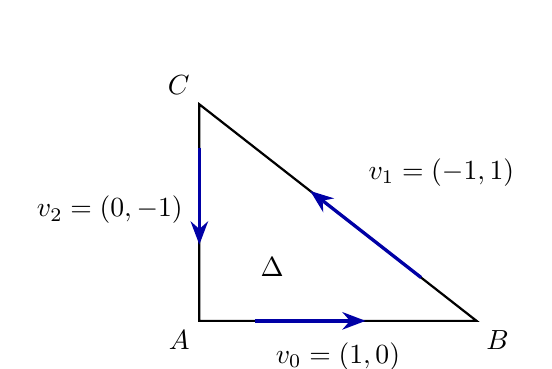
\begin{tikzpicture}[scale=2.2,>=Stealth]
\draw[thick] (0,0)--(1.6,0)--(0,1.25)--cycle;
\draw[->,very thick,blue!65!black] (.32,0)--(.96,0);
\draw[->,very thick,blue!65!black] (1.28,.25)--(.64,.75);
\draw[->,very thick,blue!65!black] (0,1)--(0,.44);
\node[below left] at (0,0) {$A$};
\node[below right] at (1.6,0) {$B$};
\node[above left] at (0,1.25) {$C$};
\node[below] at (.8,-.07) {$v_0=(1,0)$};
\node[above right] at (.92,.72) {$v_1=(-1,1)$};
\node[left] at (-.04,.64) {$v_2=(0,-1)$};
\node at (.42,.31) {$\Del$};
\end{tikzpicture}
\end{center}

Only the directions in this diagram matter; the drawing is schematic. Along $AB$, $BC$ and $CA$ respectively, use the angle functions
\begin{equation}\label{eq:theta}
\theta_0=0,\qquad
\theta_1=\frac\pi2-\At\!\left(\frac{b-a}{c}\right),\qquad
\theta_2=\frac{3\pi}2-\At\!\left(\frac bc\right).
\end{equation}
Indeed the corresponding orthonormal direction vectors are
$(a,0)$, $(b-a,c)$, and $(-b,-c)$; their angles lie respectively at $0$, in $(0,\pi)$, and in $(\pi,2\pi)$. Differentiating \eqref{eq:theta} gives
\begin{equation}\label{eq:thetaDerivative}
\dot\theta_j=\frac{\det(z,\dot z)}{|z|^2}.
\end{equation}
For the upper-half-plane branch, this follows by differentiating
$\pi/2-\At(x/y)$; the result is $(x\dot y-y\dot x)/(x^2+y^2)$. The lower-half-plane branch has the same derivative. Consequently \eqref{eq:kg} becomes
\begin{equation}\label{eq:kgAngle}
k_g\dd s=\dd\theta_j+\omega
\quad\text{on side }j.
\end{equation}

The exterior corner turns are
\begin{equation}\label{eq:betas}
\beta_B=\theta_1(B),\quad
\beta_C=\theta_2(C)-\theta_1(C),\quad
\beta_A=2\pi-\theta_2(A).
\end{equation}
All lie strictly between $0$ and $\pi$. For the middle one, write
\[
\beta_C=\pi+\At((b-a)/c)-\At(b/c).
\]
Since $a/c>0$, strict monotonicity gives the upper bound $\beta_C<\pi$; the range of $\At$ gives the lower bound $\beta_C>0$. The other two bounds follow immediately from that range.

The interior angles $\alpha_v=\pi-\beta_v$ therefore have the explicit formulas
\begin{equation}\label{eq:alphas}
\begin{aligned}
\alpha_A&=\pi/2-\At(b_A/c_A),\\
\alpha_B&=\pi/2+\At((b_B-a_B)/c_B),\\
\alpha_C&=\At(b_C/c_C)-\At((b_C-a_C)/c_C).
\end{aligned}
\end{equation}
They are the usual unsigned angles of the metric tangent sectors: $B_g$ is an isometry into an ordinary Euclidean plane, and each image sector has opening below $\pi$. The angular one-form is unchanged by an oriented orthogonal map and changes sign under a reflection. Hence its positive sector integral, and therefore each unsigned $\alpha_v$, is independent of the chosen orthonormal coordinates. This also proves the invariance needed in the vertex gluing argument.

\begin{lemma}[Turning by finite cancellation]\label{lem:turning}
The side angle changes and corner turns satisfy
\[
\sum_{j=0}^2\bigl(\theta_j(\mathrm{end})-\theta_j(\mathrm{start})\bigr)
+\beta_A+\beta_B+\beta_C=2\pi.
\]
\end{lemma}
\begin{proof}
The nonzero side changes are
$\theta_1(C)-\theta_1(B)$ and $\theta_2(A)-\theta_2(C)$.
Add \eqref{eq:betas}; every endpoint term cancels. This is an identity involving finitely many values, not an application of a theorem about arbitrary closed curves.
\end{proof}

\subsection{The local theorem}

\begin{theorem}[Gauss--Bonnet on one coordinate triangle]\label{thm:triangle}
For every coframe presentation satisfying the stated quantitative contracts,
\begin{equation}\label{eq:triangle}
\boxed{\quad
C_T+G_{T,AB}+G_{T,BC}+G_{T,CA}
=\alpha_A+\alpha_B+\alpha_C-\pi.\quad}
\end{equation}
This is an equality of effective names, with PR bounds for every required precision.
\end{theorem}
\begin{proof}
By \cref{lem:curvature} and the finite Green argument,
$C_T=-\int_{\partial\Del}\omega$.
By \cref{lem:boundary}, \eqref{eq:thetaDerivative}, and the finite FTC,
\[
\sum_eG_{T,e}
=\sum_j\bigl(\theta_j(\mathrm{end})-\theta_j(\mathrm{start})\bigr)
+\int_{\partial\Del}\omega.
\]
Add these equations and apply \cref{lem:turning}. The result is
$C_T+\sum_eG_{T,e}=2\pi-\sum_v\beta_v
=\sum_v\alpha_v-\pi$.
Every equality is backed either by finite rational algebra or by an explicit arbitrary-precision estimate already proved.
\end{proof}

\paragraph{An efficient numerical realization.}
The geodesic-curvature integral need not be evaluated by directly integrating the quotient in \eqref{eq:kg}. Compute it as
\[
\widehat G_{T,e}
=\widehat\theta_j(\mathrm{end})-\widehat\theta_j(\mathrm{start})
+\text{a rational quadrature of }\omega\text{ on }e.
\]
The finite FTC proves that this is a name of the same geometric integral. Reuse identical angle and $\pi$ approximations in \eqref{eq:alphas}. Then the angle telescope is exact even for the rational approximations, and the numerical face residual comes entirely from the finite Green estimate. One may use the boundary tags inherited from the square grid; different tags on paired faces are harmless because the explicit Riemann modulus bounds the resulting seam residual.

\section{Gluing, Euler characteristic, and a finite error theorem}\label{sec:global}

\subsection{The general triangle-metric identity}

\begin{proof}[Proof of \cref{thm:piecewise_intro}]
Sum \eqref{eq:triangle} over all faces:
\[
\sum_TC_T+\sum_{T,e}G_{T,e}
=\sum_{T,v}\alpha_{T,v}-F\pi.
\]
Reindex the corner sum by vertices and add the defect and turn terms. By their definitions,
\[
\sum_{v\text{ interior}}D_v+\sum_{v\text{ boundary}}\tau_v
=(2V_i+V_b)\pi-\sum_{T,v}\alpha_{T,v}.
\]
The angle terms cancel. The remaining value is
$(2V_i+V_b-F)\pi=2\chi\pi$ by \cref{lem:incidence}.
Finally reindex the face-side sum as one term for each boundary edge and a pair for each interior edge. This gives \eqref{eq:piecewise}. Every reindexing is a permutation of an explicitly finite list, so it is justified by finite addition.
\end{proof}

This proof makes the distinction between a cone singularity and a smooth point visible. Merely requiring equal tangential metrics on a shared edge does not imply zero vertex defect: a Euclidean cone is an immediate example. The next two lemmas use the additional smooth presentation data.

\subsection{Smooth cancellation and the fan calculation}\label{sec:gluing}

\begin{lemma}[Interior-edge cancellation]\label{lem:seam}
At an interior edge with the common metric chart specified in \cref{sec:compatibilitydata},
\[
G_{T,e}+G_{T',e}=0.
\]
This remains true for orientation-reversing coordinate changes.
\end{lemma}
\begin{proof}
The metric identity and its first derivatives imply the connection transformation identity
\begin{equation}\label{eq:connectiontransform}
\partial_{ij}\phi^\alpha+
\Gamma'{}^\alpha_{\beta\gamma}(\phi)
\partial_i\phi^\beta\partial_j\phi^\gamma
=\partial_k\phi^\alpha\Gamma^k_{ij},
\end{equation}
where repeated indices range only over $1,2$. One proof is to push forward the connection from \cref{lem:curvature}. It is metric-compatible by differentiating the pullback metric identity, and torsion-free because $\partial_{ij}\phi=\partial_{ji}\phi$. Uniqueness, proved by \eqref{eq:Christoffel}, gives \eqref{eq:connectiontransform}. Equivalently, substitute \eqref{eq:Christoffel} and clear the explicitly positive metric denominators; the identity is the same finite algebra.

Consequently the intrinsic acceleration $\nabla_TT$ of the edge is the same in the common chart whether computed from either face. Choosing the opposite unit tangent does not change this acceleration. The two inward unit conormals are opposite, because the faces lie on opposite sides of the edge. Their scalar products with the common acceleration therefore sum to zero. The arclength density is the same, since the tangential metrics agree. Integrating the pointwise identity proves the lemma. If parameters are reversed, substitute $t\mapsto1-t$ in finite tagged sums; no existence statement about reparametrization is needed.

No sign of $\det D\phi$ was used. This is why the proof does not require global orientability. Notice also that the coordinate-dependent one-forms $\omega_T$ need not cancel across an edge. It is the full geodesic-curvature term, including the angle derivative, that is intrinsic and cancels.
\end{proof}

\begin{lemma}[A certified one-turn fan has angle sum $2\pi$]\label{lem:fan}
At an interior vertex with the finite fan certificate of \cref{sec:compatibilitydata},
\[
\sum_{T\ni v}\alpha_{T,v}=2\pi.
\]
At a boundary vertex the sum is the actual opening angle of the certified sector, and it equals $\pi$ at a smooth boundary point.
\end{lemma}
\begin{proof}
Apply the Cholesky map of the common tangent metric to all rays. It preserves metric angles and has positive determinant. If the image of the reference ray is $(p,q)$, multiply further by
\[
C=\begin{pmatrix}p&q\\-q&p\end{pmatrix}.
\]
This sends the reference ray to the positive horizontal axis. Since
$C^{\mathsf T}C=(p^2+q^2)I$, it preserves angles and orientation. Thus all the determinant and half-plane order certificates remain valid.

Write each transformed ray as $(x_j,y_j)$. By the supplied margins $y_j\ne0$, and define its branch angle by
\[
\varphi_j=
\begin{cases}
\pi/2-\At(x_j/y_j),&y_j>0,\\
3\pi/2-\At(x_j/y_j),&y_j<0.
\end{cases}
\]
The upper branch takes values in $(0,\pi)$ and the lower branch in $(\pi,2\pi)$. Within either half-plane,
\[
\det(w_j,w_{j+1})
=y_jy_{j+1}\left(\frac{x_j}{y_j}-\frac{x_{j+1}}{y_{j+1}}\right)>0
\]
implies $\varphi_j<\varphi_{j+1}$ by strict monotonicity of $\At$. At the upper-to-lower transition the order is automatic, and the same determinant inequality shows that the angle difference is below $\pi$. The closing lower-to-upper difference uses $\varphi_0+2\pi$ and again lies below $\pi$.

The common tangent isometries identify these consecutive smaller sectors with the triangle interior angles defined in \eqref{eq:alphas}. Summing the branch differences once around the certified list gives exactly $2\pi$. The order certificate is essential: positive determinants between consecutive rays alone would allow a list that winds around more than once.

For a boundary vertex the list is open, with the cut in the omitted sector. Its sum telescopes to the difference of the endpoint branch angles, precisely the interior opening. At a smooth boundary point the endpoint rays are opposite. Their ratios $x/y$ are equal and their half-plane labels differ, so the two branch angles differ by $\pi$. This proves the last assertion.
\end{proof}

\begin{proof}[Proof of the geometric equality in \cref{thm:main}]
Apply the piecewise identity. \Cref{lem:seam} makes every interior seam term zero. \Cref{lem:fan} makes every interior vertex defect zero and identifies each boundary term with the signed exterior turn $\pi-\alpha_v$. The remaining identity is \eqref{eq:main}. The quantitative implementation is given next and in \cref{sec:arithmetic}.
\end{proof}

\subsection{The finite rational assembly theorem}\label{sec:assembly}

This is a useful theorem independently of the analytic origin of the data. Let $p\in\Q$ be arbitrary; it need not already be an approximation to $\pi$. Supply rational tables
\[
c_T,\quad g_{T,e},\quad a_{T,v},\quad t_v\ (v\text{ on the boundary}).
\]
Define the local residuals
\begin{align*}
r_T&=c_T+\sum_{e\subset T}g_{T,e}+p-\sum_{v\subset T}a_{T,v},\\
j_e&=g_{T,e}+g_{T',e}\quad(e\text{ interior}),\\
s_v&=\sum_{T\ni v}a_{T,v}-2p\quad(v\text{ interior}),\\
s_v&=\sum_{T\ni v}a_{T,v}+t_v-p\quad(v\text{ boundary}).
\end{align*}

\begin{theorem}[Exact residual identity and stability]\label{thm:assembly}
For every certified mesh and every such rational table,
\begin{equation}\label{eq:residualidentity}
\boxed{\quad
\sum_Tc_T+\sum_{e\text{ boundary}}g_e+\sum_{v\text{ boundary}}t_v-2p\chi
=\sum_Tr_T-\sum_{e\text{ interior}}j_e+\sum_vs_v.\quad}
\end{equation}
If the face, edge, interior-vertex, and boundary-vertex residuals are bounded respectively by $\eps_f,\eps_e,\eps_i,\eps_b$, then
\begin{equation}\label{eq:stability}
\abs{\sum_Tc_T+\sum_{e\text{ boundary}}g_e+\sum_{v\text{ boundary}}t_v-2p\chi}
\le F\eps_f+E_i\eps_e+V_i\eps_i+V_b\eps_b.
\end{equation}
Both statements are uniform theorems of finite rational arithmetic in \ipra.
\end{theorem}
\begin{proof}
Let $C,B,I,A,\Theta$ be respectively the total face-curvature, boundary-edge, interior edge-pair, corner-angle, and boundary-turn sums. Then
\[
\sum_Tr_T=C+B+I+Fp-A,
\quad \sum_vs_v=A+\Theta-(2V_i+V_b)p.
\]
Subtract $I$ from their sum. The remaining expression is
$C+B+\Theta+(F-2V_i-V_b)p=C+B+\Theta-2p\chi$
by \eqref{eq:incidence}. This proves \eqref{eq:residualidentity}.
For \eqref{eq:stability}, use $|x+y|\le|x|+|y|$ successively through the finite sums. An induction invariant bounds the absolute value of the processed partial sum by the processed number of terms times its prescribed tolerance. After clearing denominators it is quantifier-free.
\end{proof}

This theorem does not infer correct geometry from small residuals. It states exactly what any finite certificate proves: the global rational error follows from the checked local rational errors. The analytic sections prove that valid effective smooth presentations produce these certificates at every precision. That separation is also the most useful Lean architecture.

\section{The precise \ipra\ theorem and its precision schedule}\label{sec:arithmetic}

\subsection{A numerical endpoint}

Let $\operatorname{Valid}(d)$ abbreviate the first-order arithmetic presentation hypotheses: the finite mesh tests, regularity and quantitative jet contracts, positive margins, metric compatibility identities, and fan certificates. The evaluator and modulus programs occurring in this formula are fixed in advance. Their numerical parameters, including all face and chart indices, are part of $d$.

For a positive integer $m$ write $\ell(m)=\ceilLog(m)$. Define
\begin{equation}\label{eq:schedule}
\begin{aligned}
N_0&=F+E_i+V_i+V_b,\\
W&=1+N_0+2|\chi|,\\
s&=n+3+\ell(W),\\
q&=s+4+\ell(3F+8),\qquad \delta=2^{-s},\quad\eta=2^{-q}.
\end{aligned}
\end{equation}
Evaluate each face-curvature, face-side, corner-angle, and boundary-turn name to error at most $\eta$, using the routines proved above and below. Set $p=\Pi(q)$. Their values are the rational tables $c_T,g_{T,e},a_{T,v},t_v$ of \cref{sec:assembly}.

\begin{theorem}[Arithmetic Gauss--Bonnet]\label{thm:arith}
For every fixed PR presentation suite there is a primitive recursive rational function
\begin{equation}\label{eq:Z}
Z(d,n)=\sum_Tc_T+
\sum_{e\text{ boundary}}g_e+
\sum_{v\text{ boundary}}t_v-2\chi\Pi(q)
\end{equation}
such that \ipra\ proves
\begin{equation}\label{eq:ariththeorem}
\forall d\;\bigl(\operatorname{Valid}(d)\longrightarrow
\forall n\;|Z(d,n)|\le2^{-n}\bigr).
\end{equation}
All rational operations and the final inequality are interpreted on natural-number codes. The constants in \eqref{eq:schedule} are conservative.
\end{theorem}
\begin{proof}
Each exact local face identity has eight contributions to its approximation error: one curvature, three sides, one $\pi$, and three angles. Thus its numerical residual is at most $8\eta$. A paired smooth edge has residual at most $2\eta$. At an interior vertex of degree $d_v$, the residual is at most $(d_v+2)\eta$; at a boundary vertex it is at most $(d_v+2)\eta$. Here $d_v\le3F$. Our choice of $q$ makes each of these smaller than $\delta/8$.

These error comparisons can be obtained directly from the finite Green, angle and gluing proofs, rather than by treating their exact-name interpretation as an extra axiom. In the local routines below take $r=q+8$. For a vertex calculation with $d_v$ terms, call its scalar subroutines with an additional $\ell(d_v+2)$ bits. Apply the same finite-count allocation to any subdivided edge. These choices leave, for example, another $\delta/8$ of slack for the name-contract witnesses. Therefore each rational local residual is at most $\delta$. No undecidable assertion about a real value is tested by the program.

Apply \cref{thm:assembly} with all four tolerances equal to $\delta$. It gives
\[
|Z(d,n)|\le N_0\delta
\le W\,2^{-(n+3+\ell(W))}
\le2^{-(n+3)}\le2^{-n}.
\]
The proof works for arbitrary $n$; universal introduction closes that variable without induction on precision. All inductions used to justify the finite sums and bounds use quantifier-free running invariants, as detailed below.
\end{proof}

The small extra precision in \eqref{eq:schedule} also controls the approximation of the displayed geometric quantities themselves. Since $E_b=V_b$, there are $F+2V_b$ numerical terms on the left of \eqref{eq:main}; their total evaluation error is at most $(F+2V_b)\eta$. The right side has error at most $2|\chi|\eta$. These bounds tend to zero with an explicit PR rate. Thus \eqref{eq:ariththeorem} is exactly the effective-name interpretation of \eqref{eq:main}, not merely a collection of unrelated approximate identities.

\subsection{How each integral routine chooses a finite grid}

The bounds of \cref{sec:bounds} give a bound $14H^6$ for $\rho$ and a modulus $\nu_\rho$ for
$f(u,v)=(1-u)\rho(\Phi(u,v))$. The elementary jet-operation rules give Taylor moduli $\lambda_A,\lambda_B$ for the square coefficients in \eqref{eq:pullback}. Boundary connection coefficients have first derivatives bounded by a fixed multiple of $H^6$; the combined four-side bound $80H^6$ suffices.

For a local target precision $r$, a sufficient grid exponent is
\begin{equation}\label{eq:gridexp}
m=\max\left\{
\nu_\rho(r+8)+2,\ \lambda_A(r+8),\ \lambda_B(r+8),\
r+8+\ell(80H^6+1)\right\},\qquad N=2^m.
\end{equation}
The first entry controls two-dimensional cell oscillation; the second and third control the two finite differences in Green's formula; the last controls the boundary tagged quadrature error. A corresponding one-dimensional expression supplies every other integral, including those in the angle evaluator. The $+2$ is deliberately enough for the $\ell^1$ cell diameter and the triangle pullback.

Evaluate coframe jets on this grid with
\begin{equation}\label{eq:evalbits}
p_{\mathrm{jet}}=r+m+20+7\ell(2H).
\end{equation}
The stability bounds in \cref{sec:bounds} ensure that all derived coefficients used in the finite difference proof have error far below $2^{-(r+8)}/N$. Thus intermediate cancellation and rounding are accounted for explicitly. This extra $m$ in evaluation precision is important even though the final derivative-remainder error in \eqref{eq:greenerror} does not grow with $N$.

For a ratio entering an angle, $|(b-a)/c|\le2H^2$ and $|b/c|\le H^2$. Use $R=2H^2+1$ in the arctangent quadrature bound. Finite vertex fan calculations have their own supplied denominator margins; the same addition/product/reciprocal compiler determines their required precision. A finite maximum over the vertex list is a PR function of the numerical parameters.

These bounds are intended to certify primitive recursiveness, not computational efficiency. The grids may be very large when an input modulus is poor. No polynomial-time claim is made. For concrete polynomial, rational, or elementary metrics one should simplify primitives or use sharper certified quadrature, as the examples do.

\subsection{Why only quantifier-free induction is used}

The whole calculation can be organized into the following elementary finite proof blocks.
\begin{center}
\begin{tabular}{p{0.25\linewidth}p{0.64\linewidth}}
\toprule
Block & Quantifier-free invariant or proof step\\
\midrule
Mesh incidence & Equality of processed face-side counts and accumulated edge multiplicities.\\
Riemann comparison & Upper and lower bounds on a weighted processed sum.\\
One-dimensional FTC & Endpoint increment minus processed derivative sum is bounded by processed length times the cell error.\\
Discrete Green & A processed rectangular difference sum equals its remaining boundary terms.\\
Angle telescope & Equality of a processed sum of branch differences with the endpoint difference.\\
Residual assembly & A processed total differs from its expected reindexing by the explicitly accumulated residual.\\
Error bound & Absolute processed error is bounded by the sum of nonnegative processed allowances.\\
\bottomrule
\end{tabular}
\end{center}

Each running sum is a PR function symbol. Rational comparisons are cleared by positive common denominators, and signed integers are represented by differences of naturals. The resulting invariants are equalities or inequalities of natural-number terms, combined by propositional connectives and guards such as $j\le N$. Finite tables are accessed by PR decoding functions. Nested loops can be flattened into a loop of length $N^2$ with quotient/remainder indices.

The input contract may contain number quantifiers. It is never placed inside an induction formula. At a step, universal elimination instantiates it at the current rational grid points and the chosen precision, yielding the one numerical cell estimate needed by that step. If a certificate uses a bounded list of tests, its conjunction is represented by a primitive recursive Boolean fold, not by invoking an unrestricted induction schema for formulas with quantifiers. This is the same disciplined use of guarded numerical invariants seen in the inspected \repo\ module \code{TaggedFTC.lean} \cite{repo-ftc}.

Algebraic differentiation and metric invariance are finite identities between rational expressions in fixed-size jet tuples. Their denominators have the supplied positive lower bounds. Multiplication by those denominators reduces the identities to polynomial arithmetic. The irrational-looking constants arise only as rational-name programs, chiefly the explicit $\At$ integral and $\Pi$. Therefore they introduce no additional sort or axiom into \ipra.

\subsection{Total programs and hypotheses}

All arithmetic programs are total on numerical codes. A malformed rational denominator, a failed finite mesh test, or an absent positive margin can be assigned a default output, for example zero. On valid inputs the guards prove that those defaults are never used. Division in a valid geometric expression is performed only after the requested precision guarantees a rational denominator of magnitude at least half its supplied lower bound.

There are three distinct assertions worth keeping separate.
\begin{enumerate}
\item \textbf{Uniform finite theorem.} Any rational tables satisfying the finite residual checks obey \eqref{eq:stability}. This has no analytic hypotheses.
\item \textbf{Conditional smooth theorem schema.} For each fixed PR presentation suite, the arithmetic validity hypotheses imply \eqref{eq:ariththeorem}. This is what the full human proof establishes.
\item \textbf{An unconditional concrete instance.} To derive a closed theorem for a particular supplied surface in \ipra, one must additionally prove its jet contracts, margins, and gluing data in \ipra. Externally correct but unproved input contracts do not automatically supply those derivations.
\end{enumerate}
The archive's exact rational tests and symbolic examples are useful implementation checks. They do not replace the missing Lean object-language proofs of these contracts or of the general analytic blocks.

\subsection{Why the hypotheses are mathematical content, not the conclusion}

No input field asserts Gauss--Bonnet, Green's theorem, an integrated curvature identity, or a $2\pi$ interior angle sum. The input fields are local value/derivative contracts, nonsingularity and metric compatibility, and finite incidence and fan order. Green's formula is proved by the rectangular telescope; the angle sum is proved by the branch telescope; the Euler coefficient is proved by incidence counting. These three separate derivations are the mathematical content of the theorem.

The geometric restrictions also explain its constructive scope. We supply a finite atlas, moduli, and bounds instead of extracting them from qualitative compactness. We supply effective common charts instead of applying an unquantified inverse-function or triangulation theorem. We supply no solutions of geodesic differential equations: the coordinate edges may be arbitrary curved edges in the surface. Geodesic edges are an optional specialization, not a prerequisite for the proof.

\section{Consequences and worked examples}\label{sec:examples}

\subsection{A curved conformal triangle with exact rational integrals}

On $\Del$ let
\[
u(x,y)=x^2+2xy+3y^2,\qquad
g=e^{2u}(\dd x^2+\dd y^2).
\]
Then $a=c=e^u$, $b=0$, and
\[
\omega=-(2x+6y)\dd x+(2x+2y)\dd y,
\qquad \rho=-8.
\]
Thus $C_T=-8\operatorname{area}(\Del)=-4$.
The angle functions on each straight side are constant because the metric is conformal. Direct rational integration on the three parameter intervals gives
\[
G_{AB}=\int_0^1-2t\dd t=-1,
\]
\[
G_{BC}=\int_0^1(4+4t)\dd t=6,
\qquad
G_{CA}=\int_0^1-2(1-t)\dd t=-1.
\]
Their sum is $4$, so the curvature and smooth boundary integrals cancel. The interior angles are $(\pi/2,\pi/4,\pi/4)$, and the three exterior turns sum to $2\pi$. Hence
\[
-4+(-1+6-1)+2\pi=2\pi,
\]
as required for a disk. This example has nonzero smooth Gaussian curvature: it is not a Euclidean cone calculation.

The coframe is effectively presented by the ordinary rational Taylor name for the exponential. On the triangle, $0\le u\le3$ and $1\le e^u<27$; derivative bounds follow by differentiating the fixed quadratic. On the collar
$x,y\ge-1/100$, $x+y\le1+1/100$, one has
$u=(x+y)^2+2y^2<4$, $|u_x|<3$, $|u_y|<7$.
Using $e^4<81$ bounds every coframe jet through order two by $8192$, and $a,c\ge1$. The third derivatives have similarly explicit bounds, which give the required Taylor and continuity moduli. Exponential Taylor tails, bounded for example by a geometric tail once the term ratio is at most $1/2$, give a PR evaluator and all these elementary contracts. The archive checks the displayed integrals with exact fractions.

\subsection{A spherical octant, including an independent area integral}

Let $w=1-u-v$, $s=u^2+v^2+w^2$, and
\[
X(u,v)=\frac{(u,v,w)}{\sqrt s},\qquad (u,v)\in\Del.
\]
Its image is the positive octant of the unit sphere. Put
$t_1=u-w$, $t_2=v-w$, and
$A=\left(\begin{smallmatrix}2&1\\1&2\end{smallmatrix}\right)$.
Differentiation gives
\begin{equation}\label{eq:spheremetric}
g_{ij}=\frac{A_{ij}}s-\frac{t_it_j}{s^2},
\qquad \det g=s^{-3}.
\end{equation}
In particular,
\[
E=\frac2s-\frac{(u-w)^2}{s^2},\quad
F_0=\frac1s-\frac{(u-w)(v-w)}{s^2},\quad
G=\frac2s-\frac{(v-w)^2}{s^2}.
\]
All denominators have a simple rational margin: $s\ge1/3$ because
$3(u^2+v^2+w^2)\ge(u+v+w)^2=1$.

Here is an intrinsic curvature calculation that does not assume Gauss--Bonnet. Since $s_i=2t_i$ and $\partial_i t_j=A_{ij}$, the Christoffel symbols are
\[
\Gamma^k_{ij}=-\frac{\delta_i^kt_j+\delta_j^kt_i}{s}.
\]
They can be checked either in \eqref{eq:Christoffel} or by differentiating $X$ twice:
$X_{ij}=-(t_i/s)X_j-(t_j/s)X_i-g_{ij}X$.
For $q_i=t_i/s$ one has
$\partial_jq_k+q_jq_k=A_{jk}/s-t_jt_k/s^2=g_{jk}$.
Substitution into the curvature formula therefore gives
\[
R(\partial_i,\partial_j)\partial_k
=g_{jk}\partial_i-g_{ik}\partial_j.
\]
Thus $K=1$ and $\rho=\sqrt{\det g}=s^{-3/2}$. For a straight coordinate side with constant velocity $v$, the covariant acceleration in coordinate components is
$\Gamma(v,v)=-2(q\cdot v)v$, parallel to its velocity. Its unit-speed covariant acceleration vanishes, so each side is a geodesic. At each corner the two outgoing image tangents are orthogonal, giving three interior angles $\pi/2$.

We can integrate $\rho$ independently. For fixed $u$, completing the square in $v$ and differentiating the resulting elementary primitive gives
\[
\int_0^{1-u}s^{-3/2}\dd v
=\frac{2(1-u)}{\bigl(2u^2+(1-u)^2\bigr)\sqrt{u^2+(1-u)^2}}.
\]
For completeness, if $y=v-(1-u)/2$ and $A_u=2u^2+(1-u)^2$, then
$s=2y^2+A_u/2$ and a primitive is $2y/(A_u\sqrt s)$.
Now put
\[
z(u)=\frac{u}{\sqrt{u^2+(1-u)^2}}.
\]
The displayed one-variable integrand is $2z'(u)/(1+z(u)^2)$. Since $z(0)=0$ and $z(1)=1$, the finite FTC and the arctangent definition give
\[
\int_\Del\rho\dd u\dd v=2\At(1)-2\At(0)=\pi/2.
\]
Thus the local formula reads
\[
\pi/2+0=3\pi/2-\pi.
\]
The argument never uses the total area of the sphere to establish the octant area.

The presentation has strong effective margins. On $\Del$, $1/3\le s\le1$, $E,G\le6$, and $\det g\ge1$. Also
$2s-(u-w)^2=(1-v)^2+2v^2\ge2/3$, so $E\ge2/3$, and similarly $G\ge2/3$. The $2\times2$ principal-minor test gives $g\ge(1/12)I$: the shifted diagonal entries are positive and
\[
\det(g-(1/12)I)=\det g-\operatorname{tr}(g)/12+1/144\ge1/144>0.
\]
On the rational collar $u,v\ge-1/100$, $u+v\le1+1/100$, all of $u,v,w$ lie in $[-1/100,102/100]$, giving $1/3\le s\le2$. There $\det g\ge1/8$, $1/6\le E,G\le6$, and the Cholesky coefficients satisfy $a\ge1/3$, $c\ge1/7$. All higher derivative and approximation bounds come from fixed rational expressions and square roots with these positive margins. This is an actual effective smooth presentation of the required kind.

Gluing eight octants gives the round sphere with $V=6$, $E=12$, $F=8$, hence $\chi=2$. The eight curvature contributions sum to $4\pi$, seam terms vanish, and each vertex has four right-angle sectors. This also illustrates the complete smooth global calculation.

\subsection{Polyhedral and nonorientable checks}

For a constant coframe on each face, $P=Q=\rho=0$. Each face is Euclidean, so its angles sum to $\pi$. Equation \eqref{eq:piecewise} becomes
\[
\sum_{v\text{ interior}}\left(2\pi-\sum_{T\ni v}\alpha_{T,v}\right)
+\sum_{v\text{ boundary}}\left(\pi-\sum_{T\ni v}\alpha_{T,v}\right)
=2\pi\chi.
\]
For equilateral triangle metrics, every face angle is $\pi/3$, and all coefficients of $\pi$ are rational. The exact verifier checks the following meshes, their link conditions, and this identity.
\begin{center}
\begin{tabular}{lrrrrl}
\toprule
Mesh & $V$ & $E$ & $F$ & $\chi$ & Orientable\\
\midrule
Tetrahedral sphere & 4&6&4&2&Yes\\
Two-triangle disk & 4&5&2&1&Yes\\
Triangular annulus & 6&12&6&0&Yes\\
Nine-vertex torus & 9&27&18&0&Yes\\
Six-vertex projective plane & 6&15&10&1&No\\
\bottomrule
\end{tabular}
\end{center}
The projective-plane example has five equilateral sectors at each vertex, hence defect $\pi/3$ at each of six vertices and total $2\pi$. It verifies the orientation-free finite assembly, not a smooth metric claim about that particular cone metric.

The verifier also tests arbitrary rational residual tables, rejects duplicate faces and disconnected vertex links, and treats a global orientation certificate as optional. These checks target genuine failure modes of the finite formulation.

\subsection{Further consequences within the same presentation discipline}

\paragraph{Geodesic triangle excess.}
If the three supplied sides satisfy $k_g=0$, then
$\int_TK\dd A=\alpha_A+\alpha_B+\alpha_C-\pi$.
No theorem asserting the existence of geodesics is used. If $K=k$ is a constant with a supplied positive margin for $|k|$, division gives
$\operatorname{area}(T)=(\sum\alpha-\pi)/k$.

\paragraph{Closed surfaces and sign restrictions.}
For a closed smooth presentation, $\int_MK\dd A=2\pi\chi$. If the input additionally supplies $K\ge\kappa_0>0$ and a positive rational lower bound for the total area, monotonicity of the finite integral gives $\chi>0$. An everywhere negative bound gives $\chi<0$. These are constructive sign conclusions about the finite Euler characteristic; no classification theorem is imported.

\paragraph{Metric independence of total curvature.}
Any two valid smooth metric presentations on the same closed mesh have the same total curvature because each equals $2\pi\chi$. With boundary, the invariant is the sum of curvature, geodesic curvature, and corner turns. This statement includes an explicit modulus for comparing the two numerical totals.

\paragraph{Elementary refinement.}
Splitting a face by one interior vertex changes $(V,E,F)$ by $(1,3,2)$. Splitting a boundary edge and its adjacent face changes them by $(1,2,1)$; splitting an interior edge and both adjacent faces changes them by $(1,3,2)$. Each preserves $V-E+F$ by arithmetic. Effective integral additivity and the same seam/fan cancellation show that the geometric total is preserved under the corresponding supplied smooth subdivisions. A general theorem relating arbitrary abstract triangulations is not needed for these useful refinement operations.

\subsection{What the computations establish}

The included Python scripts establish exact finite arithmetic identities on their stated test instances. The spherical script additionally verifies the displayed finite symbolic formulas with SymPy and compares independent quadratures at 50-digit working precision. A displayed floating-point difference of zero is only agreement at that working precision; it is not an interval error certificate. None of these executions is described as a Lean kernel check or as an executable proof of the entire theorem schema. The human proof and its explicit error bounds supply the mathematical argument; the scripts check implementation and sign conventions.

\section{Lean formalization: definitions, reusable code, and completion path}\label{sec:lean}

\subsection{Three layers that must remain separate}

The intended endpoint is a Lean term inhabiting an object-language derivability judgment
\[
\Gamma\ \vdash[\mathrm{PRAAx}]\ \varphi,
\]
where $\Gamma$ consists of the arithmetic presentation contracts and $\varphi$ is the rational error formula. A theorem in Lean's ambient logic about $\Q$, finite sets, or $\R$ is useful for developing the argument, but does not by itself provide that judgment.

The archive therefore distinguishes:
\begin{enumerate}
\item the fully developed human proof in this report;
\item ambient finite algebra in \code{lean/Assembly.lean};
\item candidate object-level polynomial and inequality steps in \code{lean/IPRABridge.lean}, together with a detailed blueprint for the still-unimplemented analytic and finite-mesh derivations.
\end{enumerate}
No Lean executable, Lake executable, or Elan installation was available in the authoring runtime. The two source files contain no admitted proofs or new axioms, but they are \emph{uncompiled candidates}. This is not a claim that the final theorem, or even these candidate files, has been kernel-checked here.

\subsection{Definitions required for the complete development}

The following interfaces specify the data needed; they are mathematical specifications for Lean implementation, not assumed theorem fields. All evaluator programs belong to the fixed PR syntax already available in \repo\ \cite{repo-pr}.

\begin{longtable}{p{0.24\linewidth}p{0.68\linewidth}}
\toprule
Definition & Required content\\
\midrule
\endhead
\code{QCode} & A triple $(a,b,d)$ denoting $(a-b)/(d+1)$; PR equality, order, arithmetic and absolute-error checks by positive cross multiplication.\\
\code{PRRational k} & Three fixed elements of \code{PR k}, giving the two numerator parts and the denominator minus one. This is syntax for a fixed program family, not a universal evaluator.\\
\code{RegularContract} & The numerical formula \eqref{eq:regular}, with ordinary parameter variables and precision variables.\\
\code{SurfaceCode} & Face triples, edge occurrence lists, vertex link traversals, boundary flags, and finite permutation witnesses as in \cref{def:mesh}.\\
\code{surfaceOK} & A PR Boolean fold checking those lists, local degrees, and traversals.\\
\code{Counts} & $V_i,V_b,E_i,E_b,F$ and the derived equations \eqref{eq:incidence}. In an ambient prototype these may be structure fields; in the final derivation they are conclusions of \code{surfaceOK}.\\
\code{JetSuite} & The 18 coframe jet entries: three fields $a,b,c$, each with multi-indices $0,x,y,xx,xy,yy$; common bound $H$ and fixed modulus programs.\\
\code{C2Contract} & Regularity, positivity, bounds, continuity \eqref{eq:continuitycontract}, and Taylor inequalities \eqref{eq:jetcontract}, all expanded to numerical formulas.\\
\code{FrameFields} & The explicit rational expressions $P,Q,P_i,Q_i,\rho$ of \eqref{eq:PQ} and \eqref{eq:rho}, with syntactically generated derivative expressions.\\
\code{AtApprox}, \code{PiApprox} & The bounded rational quadrature in \eqref{eq:At}, with explicit grid length and approximation bounds.\\
\code{TriangleIntegral} & The square-grid evaluator of $(1-u)\rho(\Phi(u,v))$ using \eqref{eq:gridexp}.\\
\code{SideIntegral} & The endpoint angle difference plus the tagged connection integral proved equivalent to \eqref{eq:kg}.\\
\code{CornerAngle} & The three branches in \eqref{eq:alphas}, with shared endpoint evaluations where useful.\\
\code{EdgeContract} & Common chart jets, metric first-jet identities, parameter matching, positive speed/Jacobian margins, and opposite transverse determinant signs.\\
\code{FanCertificate} & Common tangent metric, differential identifications, half-plane labels, ordered ray lists, and strict determinant margins; no angle-sum field.\\
\code{BoundaryTurn} & $\pi$ minus the certified opening angle, computed by its branch telescope.\\
\code{ResidualTables} & The four rational residual arrays of \cref{sec:assembly}.\\
\code{Valid}, \code{Defect} & The conjunction of input contracts and the PR rational function $Z(d,n)$ of \eqref{eq:Z}.\\
\bottomrule
\end{longtable}

This makes every mathematical object in the final theorem either a finite code, a fixed PR program, or a first-order contract about one. It also identifies where semantic interpretation is needed: the regular-name construction and the proofs that the frame expressions are the conventional Gaussian and geodesic curvatures. Those interpretation proofs have already been given mathematically in \cref{sec:calculus,sec:local}.

\subsection{The supplied ambient algebra candidate}

The central statement in \code{Assembly.lean} uses an arbitrary rational $p$, so it does not hide an assumption about $\pi$. In abbreviated form it is:
\begin{lstlisting}
theorem assembly_identity (c : Counts)
    (p C B I A Theta : Rat) :
    C + B + Theta - 2 * p * c.eulerQ =
      faceResidual c p C B I A - I +
      vertexResidual c p A Theta := by
  -- cast the two natural incidence equalities to rationals
  -- unfold the three explicit polynomial expressions
  -- take the combination -p * incidence + p * boundary
\end{lstlisting}
The actual file supplies the tactic proof, the absolute-error bound, the polyhedral specialization, and sample mesh counts. This layer checks the finite algebra once a Lean toolchain is available. It does not prove that the geometry supplies the residual hypotheses.

The candidate \code{IPRABridge.lean} targets the repository's actual \code{PRAAx} judgments for a sign-free Euler-coefficient polynomial and upper/lower three-term error combination. It uses the inspected arithmetic APIs \code{natEq}, \code{deriveNat}, and \code{ipra_le}. Its scope is intentionally small: variable-length counting, grid calculations, and analytic interpretation remain separate modules to write.

\subsection{Existing \repo\ results that can be reused}

We inspected commit \code{d36b35eed5bd01af4ade66bf539622495813ccc8}. Its README distinguishes the checked derivation libraries from delivered research packets \cite{repo-readme}. We did not rebuild that repository in this runtime.

\begin{itemize}
\item \code{Analysis/TaggedFTC.lean} gives object-level finite telescoping and error accumulation from cell inequalities using \code{PRA.qfInd}. Its source explicitly leaves production of the derivative cell inequality and passage to names outside the module \cite{repo-ftc}.
\item \code{Analysis/RiemannSumRules.lean} gives finite-sum linearity, scaling, bounds and closeness rules with object-level conclusions \cite{repo-sums}.
\item Two further Analysis modules, \code{GridIntegral.lean} and \code{RiemannRefinement.lean}, provide one-dimensional finite comparison patterns. They do not already supply the two-dimensional Green calculation of this report \cite{repo-grid}.
\item \code{Topology/EulerCharacteristic.lean} contains an object-level finite Euler--Poincare theorem. Its separate ambient additivity lemmas do not replace the surface-link counting proof required here \cite{repo-euler}.
\item \code{Topology/BoundarySquare.lean} provides an ambient finite cancellation pattern, useful as a design reference for occurrence reindexing; it is not a Gauss--Bonnet derivation \cite{repo-boundary}.
\end{itemize}

The newer analysis and continuous-framework research packets support fixed-program names, explicit moduli and finite contracts, but should not be imported as if their application theorems were already checked. The source audit in the archive records exact paths, blob identifiers, and this distinction.

\subsection{A concrete order for completing the Lean proof}

\begin{enumerate}
\item \textbf{Finite surface arithmetic.} Implement the occurrence lists and link checks, then prove double counting and reindexing with guarded QF invariants. Integrate the candidate coefficient identity. This completes the uniform finite rational theorem \cref{thm:assembly} in the object calculus.
\item \textbf{Quantitative scalar operations.} Implement rational error propagation, the product/reciprocal Taylor rules, positive square-root approximation, and the arctangent quadrature. Prove each numerical bound as a \code{PRAAx} derivation. Keep the expression-tree compiler syntactic and fixed.
\item \textbf{Grid integration.} Extend existing finite-sum rules to flattened $N\times N$ indices. Prove \eqref{eq:discretegreen} exactly, then the two signed versions of \eqref{eq:greenerror}. Add the explicit auxiliary evaluation error $4N\eps_{\rm grid}+2\eps_{\rm derivative}$.
\item \textbf{Local differential algebra.} Encode order-two jet tuples and the finite formulas for $P,Q,\rho$. Clear positive denominators and prove the torsion, connection and curvature identities. Construct the Taylor-modulus proofs using the scalar-operation lemmas, rather than asking for the curvature formula as an interface assumption.
\item \textbf{Angles and boundary curvature.} Prove the arctangent derivative, reciprocal relation, three side branches, and exact endpoint telescope. Derive the side-integral name from the finite FTC. Combine with the grid theorem to obtain the local residual bound.
\item \textbf{Gluing.} Prove the connection transformation identity from the metric jet equations. Use opposite conormal signs for seam cancellation. Implement the two half-plane angle branches and the finite fan telescope; derive the vertex residual bound from order certificates.
\item \textbf{Final numerical theorem.} Substitute the PR precision schedule \eqref{eq:schedule}, call each local bound, and invoke the finite assembly theorem. The result is the object-language universal precision formula corresponding to \eqref{eq:ariththeorem}.
\item \textbf{Semantic adequacy and instances.} In a separate ambient Lean development, interpret regular names as real values and prove that the numerical expressions agree with the usual integrals and curvatures. For a closed concrete \ipra\ instance, also derive its presentation contracts. The ambient interpretation neither adds axioms to nor substitutes for the object proof.
\end{enumerate}

Every listed mathematical lemma has a proof in this report, an explicit finite computational specification, or both. The remaining work is its detailed encoding and kernel verification. A realistic completion should check each module against the pinned repository toolchain, which the inspected \code{lean-toolchain} specifies as Lean 4.32.0, and record the exact successful build command and commit. No such receipt is supplied for the new Lean files here.

\subsection{Reproduction files}

The archive includes the LaTeX source and PDF; three Python reference verifiers; their actual output records; two Lean candidates; a formalization blueprint; and the pinned source audit. The top-level \code{README.md} gives the build and verification commands. The exact tests exercise the finite arithmetic, including incorrect orientation and invalid-link cases. The symbolic smooth tests are explicitly separated from numerical diagnostics and from formal proof status.

\appendix
\section{Explicit bounds and the elementary jet compiler}\label{sec:bounds}

This appendix makes the quantitative analytic steps reproducible. Throughout, $H\ge1$ is an integer and \eqref{eq:Hbounds} holds. All norms of a jet tuple below mean the maximum absolute difference of its finitely many entries.

\subsection{Bounds for the connection and density}

Put $u=b_x-a_y$ and $w=c_x+bP$. Then
\[
|u|,|u_i|\le2H,\qquad
|w|\le3H^3,\qquad |w_i|\le7H^5,
\]
because
\[
P_i=\frac{u_i}{c}-\frac{u c_i}{c^2},\quad
w_i=c_{xi}+b_iP+bP_i,\quad
Q_i=\frac{w_i}{a}-\frac{wa_i}{a^2}.
\]
Successive substitution gives the table
\begin{center}
\begin{tabular}{lc}
\toprule
Quantity & Uniform absolute bound\\
\midrule
$P$ & $2H^2$\\
$P_x,P_y$ & $4H^4$\\
$Q$ & $3H^4$\\
$Q_x,Q_y$ & $10H^6$\\
$\rho=P_y-Q_x$ & $14H^6$\\
$k_g\,\dd s/\dd t$ on any reference side & $13H^4$\\
\bottomrule
\end{tabular}
\end{center}
For the last row, the angle density on $BC$ has numerator
$x\dot y-y\dot x$ with $x=b-a$, $y=c$,
$|x|\le2H$, $|y|\le H$, $|\dot x|\le4H$, $|\dot y|\le2H$.
Its denominator is at least $c^2\ge H^{-2}$, so its absolute value is at most $8H^4$. The $CA$ angle density is at most $2H^4$, and the $AB$ angle density is zero. The connection term is at most $5H^4$ on every side. These calculations prove the uniform bound.

\subsection{Stability with respect to rational jet approximations}

Compare two jet tuples each satisfying the same $H$ bounds, and suppose every entry differs by at most $\eps$. Then
\begin{equation}\label{eq:stabilityconstants}
\begin{aligned}
|\Delta P|&\le4H^3\eps,&
|\Delta P_i|&\le12H^5\eps,\\
|\Delta Q|&\le10H^5\eps,&
|\Delta Q_i|&\le46H^7\eps,\\
|\Delta\rho|&\le58H^7\eps.
\end{aligned}
\end{equation}
Here $\Delta$ means the difference between the two evaluations, not a derivative. The useful elementary estimates are
\[
|c^{-1}-{c'}^{-1}|\le H^2\eps,
\qquad |c^{-2}-{c'}^{-2}|\le2H^3\eps,
\]
and the same for $a$. They follow by factoring the differences, not by a mean-value theorem. Subtract products one factor at a time. This first gives
$|\Delta w|\le7H^4\eps$ and
$|\Delta w_i|\le23H^6\eps$.
The two terms of $Q_i=w_i/a-wa_i/a^2$ contribute at most
$30H^7\eps$ and $16H^7\eps$, respectively. The other rows follow directly from the formulas above.

For the $BC$ angle density, the numerator changes by at most $16H\eps$, the denominator by at most $10H\eps$, and the denominator is at least $H^{-2}$. Factoring a quotient difference gives a bound $96H^7\eps$ for its change. Including the connection term bounds the change of the entire side density by $110H^7\eps$. The other sides have smaller bounds.

For the square coefficients at a fixed rational point $(u,v)$,
\[
|\Delta A|\le14H^5\eps,\quad |\Delta B|\le10H^5\eps,
\]
\[
|\Delta A_v|\le68H^7\eps,\quad
|\Delta B_u|\le102H^7\eps.
\]
Now suppose one tuple is exact and the other comes from evaluation errors at most $\eps\le1/(2H)$. The approximate tuple satisfies the original bounds with $H'=2H$: its positive entries remain at least $1/(2H)$ and all jets are at most $2H$. Replacing $H$ by $2H$ in all the preceding estimates shows that
\begin{equation}\label{eq:universalstability}
|\Delta F|\le32768H^7\eps
\end{equation}
is a common conservative bound for every density or coefficient used in the square-grid proof and the reference-side density. Since
$2^{7\ell(2H)}\ge(2H)^7$, the evaluation precision in \eqref{eq:evalbits} makes \eqref{eq:universalstability} at most
$2^{-(r+m+12)}$, below the required $2^{-(r+8)}/N$.

\subsection{A modulus for the square integrand}

The map $\Phi$ satisfies
$\norm{\Phi(z)-\Phi(z')}_1\le2\norm{z-z'}_1$.
If the square-point distance is at most $\rho_0$ and the resulting jet differences are at most $\eps$, then
\[
\left|\Delta\bigl((1-u)\rho(\Phi)\bigr)\right|
\le58H^7\eps+14H^6\rho_0.
\]
Let $h_H=\ell(H)$ and $s_r=r+8+7h_H$. A sufficient modulus is
\begin{equation}\label{eq:nu}
\nu_\rho(r)=\max\{\mu(s_r)+2,\ s_r+2\}.
\end{equation}
At the prescribed distance, both $\eps$ and $\rho_0$ are at most $2^{-s_r}$, so the displayed bound is below $2^{-r}$. The extra two bits safely cover the $\ell^1$ pullback factor. This is a continuity modulus, not a substitute for the derivative-remainder moduli used in finite differences.

The first derivatives of the square coefficients obey
\[
|A_u|\le28H^6,\quad |A_v|\le17H^6,\quad
|B_u|\le23H^6,\quad |B_v|\le10H^6.
\]
For example, $A_u=P_x-vP_y-vQ_x+v^2Q_y$ after pullback. The corresponding boundary left-sum error is at most
$(2\cdot28+2\cdot10)H^6/N\le80H^6/N$.
The one-dimensional derivative bound implies the needed Lipschitz estimate by the finite FTC, so this argument does not introduce an unproved mean-value principle.

\subsection{Compiling Taylor witnesses by rational operations}

Here is a direct way to generate the moduli $\lambda_A,\lambda_B$ used above. Suppose $f$ has value bound $B_f$, derivative coefficient bound $D_f$, and Taylor remainder bound $\eps\norm h_1$ at a suitably small step. At a step where $\eps\le1$, it also has the increment bound
$|f(z+h)-f(z)|\le C_f\norm h_1$, where $C_f=D_f+1$.

\paragraph{Addition.}
Add the two remainder bounds and request one extra bit for each. Derivative and value bounds add.

\paragraph{Product.}
Writing $\Delta f=f(z+h)-f(z)$ and similarly for $g$,
\[
\Delta(fg)-D(fg)(z)h
=f(z)R_g+g(z)R_f+\Delta f\,\Delta g.
\]
Its absolute value is at most
\begin{equation}\label{eq:productTaylor}
(B_f+B_g)\eps\norm h_1+C_fC_g\norm h_1^2.
\end{equation}
For a target $2^{-r}\norm h_1$, it suffices to use the input moduli at
$r+2+\ell(1+B_f+B_g)$ and to impose
$\norm h_1\le2^{-(r+2+\ell(1+C_fC_g))}$.
Taking the maximum of these finitely many requirements gives a PR output modulus. Bounds may be rounded upward to integers before using $\ell$.

\paragraph{Reciprocal.}
Suppose $|f|\ge1/M$ with a fixed integer $M\ge1$. The exact identity
\[
\frac1{f+\Delta f}-\frac1f
=-\frac{\Delta f}{f^2}
+\frac{(\Delta f)^2}{f^2(f+\Delta f)}
\]
gives the remainder bound
\begin{equation}\label{eq:reciprocalTaylor}
M^2\eps\norm h_1+M^3C_f^2\norm h_1^2.
\end{equation}
Use the input modulus at $r+2+\ell(1+M^2)$ and require
$\norm h_1\le2^{-(r+2+\ell(1+M^3C_f^2))}$.
The lower bound is required at both endpoints, as is already guaranteed on the input domain. This construction works for either sign of $f$.

\paragraph{Fixed compositions.}
For a quantitative map $\psi$ with increment bound $L\norm h_1$ and Taylor remainder $\eps_\psi\norm h_1$, expand
\[
f(\psi(z+h))-f(\psi(z))
=Df(\psi(z))\bigl(\psi(z+h)-\psi(z)\bigr)+R_f.
\]
The remainder after subtracting $Df(\psi(z))D\psi(z)h$ is bounded by
$(L\eps_f+D_f\eps_\psi)\norm h_1$.
Request enough additional bits in both moduli to make this below $2^{-r}\norm h_1$, and ensure $L\norm h_1$ is within $f$'s permitted step size. The polynomial map $\Phi$ has explicit first derivatives and a quadratic remainder, so this is especially simple for the Green proof. Supplied domain margins make all evaluations legal.

Apply the Taylor rules to the fixed expression trees for $P,Q,A,B$. Obtain their first derivatives algebraically, and compile only continuity moduli for those derivative expressions. An input jet of order one has its own derivative contract with the order-two entries as derivatives. Thus the compiler uses only the given $C^2$ jets. It does not ask for third derivatives or for Taylor contracts of $P_i$ and $Q_i$.

\paragraph{Square roots, when starting with metric coefficients.}
For a named $x$ with $1/M\le x\le B$, approximate $x$ by a rational within a prescribed error so the approximation is at least $1/(2M)$. Bisect the rational interval $[0,B+1]$ a predetermined number of times to approximate its square root. Every branch compares rational squares, and the iteration bound is explicit. The identity
\[
|\sqrt x-\sqrt y|=\frac{|x-y|}{\sqrt x+\sqrt y}
\]
supplies a rational Lipschitz bound on this positive range and a PR precision schedule. Differentiation gives
\[
(\sqrt f)_i=\frac{f_i}{2\sqrt f},\qquad
(\sqrt f)_{ij}=\frac{f_{ij}}{2\sqrt f}
-\frac{f_if_j}{4f^{3/2}}.
\]
The same difference identity, followed by the product and reciprocal estimates, proves the Taylor contracts; continuity bounds follow from the displayed formulas. This justifies the effective Cholesky construction without an unbounded search or an assumption that arbitrary square roots are exact rational operations.

The angle evaluator is handled by its explicit integral and the derivative
$(1+x^2)^{-1}$, already proved in \cref{sec:calculus}. Combining these rules supplies every local bound and modulus used in the main precision schedule.

\section{Source and verification record}\label{sec:sources}

The user-specified article \cite{wiki} fixes the classical target, including boundary and corner terms. The author-hosted texts \cite{new,shifrin} provide conventional geometric context. The detailed quantitative proofs, finite-grid implementation, and proof-theoretic accounting in this report are developed here rather than attributed to those classical sources.

The \repo\ snapshot was read through the selected GitHub connection at commit
\begin{center}
\code{d36b35eed5bd01af4ade66bf539622495813ccc8}.
\end{center}
The source audit records the relevant modules' exact blob identifiers. It reports source inspection, not an independent rebuild. No existing Gauss--Bonnet module was found in the inspected derivation tree, research-packet filenames, or GitHub code search; that statement does not assert exhaustive absence from every archive in the repository.

\begin{center}
\begin{tabular}{p{0.48\linewidth}p{0.42\linewidth}}
\toprule
Item & Status in this package\\
\midrule
Human mathematical argument & Developed in full, with explicit hypotheses and error bounds.\\
Exact mesh and residual checks & Executed successfully with rational arithmetic.\\
Exact discrete FTC/Green checks & Executed successfully, including sharp bounds and negative cases.\\
Smooth examples & Exact rational and symbolic identities checked; floating-point quadratures labeled diagnostics.\\
New Lean candidate files & Not compiled; no completed formal Gauss--Bonnet derivation claimed.\\
Existing \repo\ derivations & Source inspected; existing build status recorded; not rebuilt here.\\
General effective triangulation existence & Not assumed as a theorem; finite triangulation is supplied data.\\
\bottomrule
\end{tabular}
\end{center}

\begin{thebibliography}{20}

\bibitem{wiki}
Wikipedia contributors, \emph{Gauss--Bonnet theorem}, user-specified overview.
\href{https://en.wikipedia.org/wiki/Gauss%E2%80%93Bonnet_theorem}{User-specified article}.
Consulted November 21, 2026.

\bibitem{new}
Steven New, \emph{Chapter 3. Geodesic Curvature and the Gauss--Bonnet Theorem}, PMATH 365 course notes, University of Waterloo, especially the local-to-global proof.
\url{https://www.math.uwaterloo.ca/~snew/PMATH365/Chap3GaussBonnet.pdf}.

\bibitem{shifrin}
Theodore Shifrin, \emph{Differential Geometry: A First Course in Curves and Surfaces}, April 2021, Chapter 3, sections 1 and 3.
\url{https://www.math.uga.edu/sites/default/files/inline-files/ShifrinDiffGeo.pdf}.

\bibitem{repo-readme}
Vladimir Reshetnikov and contributors, \emph{ProveIt: Primitive recursive arithmetic}, repository README at the inspected commit.
\href{https://github.com/VladimirReshetnikov/ProveIt/blob/d36b35eed5bd01af4ade66bf539622495813ccc8/Logic/PrimitiveRecursiveArithmetic/README.md}{Pinned README and verification-status table}.

\bibitem{repo-pr}
\repo, \emph{ConciseIPRA/PR.lean}: primitive recursive syntax, \code{PRAAx}, and \code{PRA.qfInd}.
\href{https://github.com/VladimirReshetnikov/ProveIt/blob/d36b35eed5bd01af4ade66bf539622495813ccc8/Logic/PrimitiveRecursiveArithmetic/ConciseIPRA/Lean/ConciseIPRA/PR.lean}{Pinned foundation source}.

\bibitem{repo-ftc}
\repo, \emph{Analysis/TaggedFTC.lean}: the finite tagged-division estimate.
\href{https://github.com/VladimirReshetnikov/ProveIt/blob/d36b35eed5bd01af4ade66bf539622495813ccc8/Logic/PrimitiveRecursiveArithmetic/Derivations/Lean/IPRADerivations/Analysis/TaggedFTC.lean}{Pinned source and its explicit scope statement}.

\bibitem{repo-sums}
\repo, \emph{Analysis/RiemannSumRules.lean}: finite Riemann-sum identities and inequalities.
\href{https://github.com/VladimirReshetnikov/ProveIt/blob/d36b35eed5bd01af4ade66bf539622495813ccc8/Logic/PrimitiveRecursiveArithmetic/Derivations/Lean/IPRADerivations/Analysis/RiemannSumRules.lean}{Pinned source}.

\bibitem{repo-grid}
\repo, \emph{Analysis/GridIntegral.lean} and \emph{Analysis/RiemannRefinement.lean}: finite one-dimensional grid comparison.
\href{https://github.com/VladimirReshetnikov/ProveIt/blob/d36b35eed5bd01af4ade66bf539622495813ccc8/Logic/PrimitiveRecursiveArithmetic/Derivations/Lean/IPRADerivations/Analysis/GridIntegral.lean}{GridIntegral source};
\href{https://github.com/VladimirReshetnikov/ProveIt/blob/d36b35eed5bd01af4ade66bf539622495813ccc8/Logic/PrimitiveRecursiveArithmetic/Derivations/Lean/IPRADerivations/Analysis/RiemannRefinement.lean}{RiemannRefinement source}.

\bibitem{repo-euler}
\repo, \emph{Topology/EulerCharacteristic.lean}: finite Euler--Poincare derivation and ambient auxiliary results.
\href{https://github.com/VladimirReshetnikov/ProveIt/blob/d36b35eed5bd01af4ade66bf539622495813ccc8/Logic/PrimitiveRecursiveArithmetic/Derivations/Lean/IPRADerivations/Topology/EulerCharacteristic.lean}{Pinned source}.

\bibitem{repo-boundary}
\repo, \emph{Topology/BoundarySquare.lean}: finite opposite-sign cancellation.
\href{https://github.com/VladimirReshetnikov/ProveIt/blob/d36b35eed5bd01af4ade66bf539622495813ccc8/Logic/PrimitiveRecursiveArithmetic/Derivations/Lean/IPRADerivations/Topology/BoundarySquare.lean}{Pinned source}.

\end{thebibliography}

\end{document}
